After showcasing the implementation of the smart contracts and the customer and ride provider frontend, the last component that is part of the prototype implementation of the GETACAR platform is the Matching Service. The matching service is written in NodeJs and the bids are stored inside MongoDB as a NoSQL database. The design decision of utilising a NoSQL database in connection with the matching service was made for several reasons. NoSQL databases provide high performance and simplify the storage of the ride requests and ride bids that are stored as simple JSON objects. Lastly, there is also no need for complex SQL functions inside the matching service that would promote the usage of an SQL database.


\subsection{Endpoints and Data}
The NodeJs application provides four core endpoints for customers and ride providers to handle all interactions with the matching service. Following ride flow, the first endpoint that is typically utilised is the POST /requestRide endpoint. The customer frontend utilises this endpoint to post ride requests to the matching service. The request contains the following data points:

\begin{itemize}
    \item \textbf{userId:} The customer pseudonym provided by an authentication service
    \item \textbf{pickupLocation:} The cloaked pickup location
    \item \textbf{dropoffLocation:} A cloaked dropoff location
    \item \textbf{userRating:} The rating of the customer
    \item \textbf{rating:} The rating of the customer requesting the ride
    \item \textbf{userPublicKey:} A newly generated public key from the customer used for the Diffie-Hellman Key Exchange
    \item \textbf{maxWaitingTime:} The maximum time the customer is willing to wait for the arrival of the ride provider
    \item \textbf{minRating:} The minimum rating necessary for a ride provider to have to be allowed to manage the ride
    \item \textbf{minPassengerRating:} The minimum rating for passengers to have to be allowed to share the ride with the customer
    \item \textbf{maxPassengers:} The maximum amount of passengers the customer is willing to have at once
\end{itemize}

The Matching Service adds the following data points to the ride request and writes them onto the database:

\begin{itemize}
    \item \textbf{rideRequestId:} A unique id to identify the ride request
    \item \textbf{gridLocation:} The grid square from where the ride request came from. This makes it easier for ride provider to find fitting ride requests if a matching service is deployed for a number of different grid squares. 
    \item \textbf{auctionStartedTimestamp:} The timestamp represents the moment the data was posted onto the matching service visibale for ride providers to bid on the ride request. 
    \item \textbf{auctionStatus:} The status of the auction. The auction can have one of four different statuses: 'open', 'determining-winner', 'waiting-for-signature' or 'closed'. 
    \item \textbf{auctionWinner:} The winner of the auction. If the winner was not determined yet, this field is empty.
    \item \textbf{winningBid:} The unique identifier of the winning bid. If the winner was not determined yet, this field is empty.
\end{itemize}

Once the complete ride request is available in the database, it can be read by ride providers. Ride providers can use the GET /rideRequests endpoint to receive a JSON object containing all ride requests with open auctions. The ride provider can search this dataset and, once they find a fitting ride request, bid on it.
To bid on a ride request, the ride provider can utilise the POST /bid endpoint. A bid request contains the following data points:

\begin{itemize}
    \item \textbf{rideRequestId:} The id of the ride request that this bid is for
    \item \textbf{rideProviderId:} The ride provider pseudonym provided by an authentication service
    \item \textbf{amount:} The maximum ride cost that the ride provider is willing to offer the ride for
    \item \textbf{rating:} The rating of the ride provider
    \item \textbf{model:} The model of the vehicle
    \item \textbf{estimatedArrivalTime:} The time to get to the customer pickup location
    \item \textbf{passengerCount:} The amount of passengers inside the vehicle when arriving at the pickup location
    \item \textbf{vehiclePublicKey:} A newly generated public key from the ride provider used for the Diffie-Hellman Key Exchange 
\end{itemize}

Before a bid can be posted to the database, the Matching Service compares the timestamp of the bid with the timestamp of the ride request the bid is associated with to ensure that the auction is truly open. For this prototype, the time frame for this is set to 30 seconds. The bid also gets extended with additional data points by the matching service itself before it gets written onto the database. These are the additional data points:

\begin{itemize}
    \item \textbf{bidId:} A unique id to identify the bid
    \item \textbf{bidPlacedTimestamp:} Timestamp representing the moment the bid is posted
\end{itemize}

With ride requests and associated bids being written to the database, the next step for the matching service is handling the running auction. Each auction is posted with the status ''open''. A function managed by the Matching Service continuously crawls the database for ride requests where the auction is older than 30 seconds. If such an auction is found, the auction status changes from 'open' to 'determining-winner'. A second function then takes the ride request and analyses all bids connected with the request to determine the winning bid based on the principles of the second price auction. The winning bid is then written into the ride request itself, changing the auction status to 'waiting-for-signature'. 

The customer is able to check the status of their auction through the GET /rideRequest/:rideRequestId endpoint by providing the identifier of their ride request inside the URL. This endpoint returns the status of the auction, and in case a winning bid was found, it additionally returns the winning bid itself. Based on the winning bid the customer can then decide if they want to take the ride or not. If the customer decides to take the ride, they follow the ride flow and create a ride contract through the contract factory that contains the maximum ride cost as a deposit. They then need to use the GET setContractAddress/:rideRequestId/:contractAddress endpoint to update their ride request with the contact's address on the blockchain. As the creation of the contract is understood as the initial signing of the ride contract, the status of the auction changes from 'waiting-for-signature' to 'closed'. 

The GET /rideRequest/:rideRequestId endpoint also enables the ride provider to track the status of the auction. Through the endpoint, the auction winner is able to receive the address of the ride contract and is, therefore, able to co-sign the contract as a ride provider.

\subsection{Grid System}
As described in \ref{subsec:MatchingService}, the design of the Matching Service includes a map grid that is utilised to assign matching services to specific jurisdiction zones and to cloak the exact pickup and dropoff locations of customers. There are many possible ways to create a map grid that would allow for this use case. The GETACAR prototype implementation uses H3, a hexagonal hierarchical geospatial indexing system that provides a predefined grid for the platform to use. The advantage of H3 is that it provides a number of grid resolutions, as each grid is made up of hexagons and pentagons that themself are made up of smaller hexagons and pentagons. An algorithm allows one to easily check if a hexagon/ pentagon of a smaller resolution is contained within a hexagon/ pentagon of a higher resolution. This approach would allow GETACAR to utilise dynamic resolutions for the  jurisdiction zones and the location cloaking with higher resolutions used for crowded areas with high traffic, like cities and lower resolutions that cover larger, less crowded  areas with less traffic. The prototype uses fixed resolutions with Res 9 for the location cloaking and Res 6 for the  jurisdiction zones of the matching services. 

\begin{figure}[h]
    \centering
    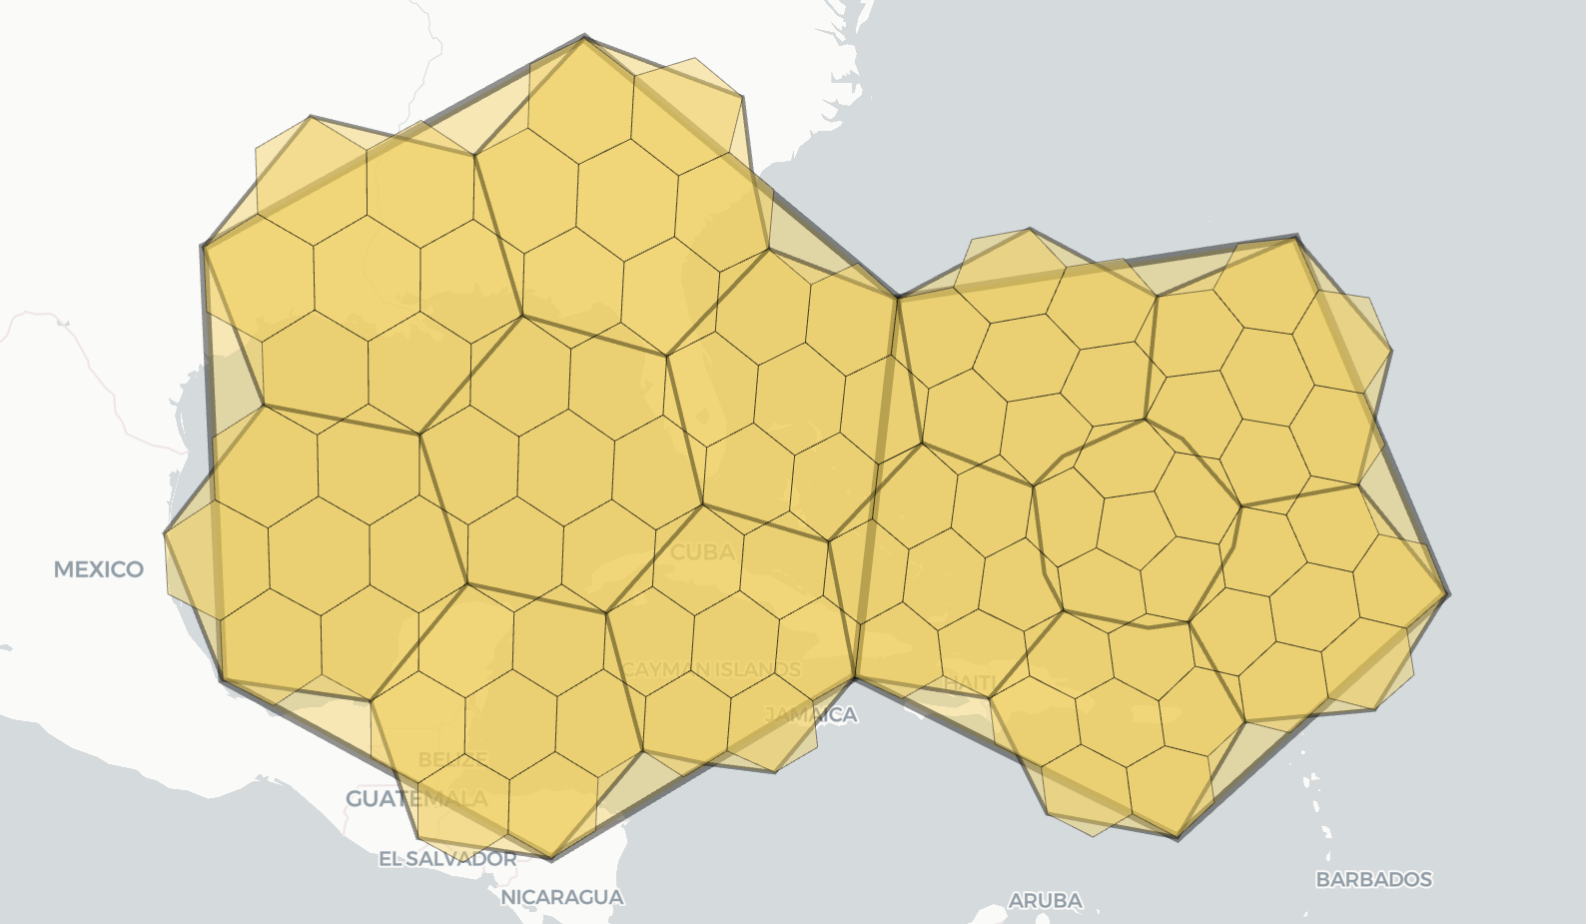
\includegraphics[width=\linewidth]{data/11.png}
    \caption{H3 Grid Visualisation}
    \label{fig:H3Visualisation}
\end{figure}

\begin{table}[h]
\centering
\begin{tabular}{|c|r|r|r|}
\hline
\textbf{Res} & \textbf{Average Hexagon Area (km$^2$)} & \textbf{Pentagon Area (km$^2$)} & \textbf{Ratio (P/H)} \\
\hline
0 & 4,357,449.416078381 & 2,562,182.162955496 & 0.5880 \\
1 & 609,788.441794133 & 328,434.586246469 & 0.5386 \\
2 & 86,801.780398997 & 44,930.898497879 & 0.5176 \\
3 & 12,393.434655088 & 6,315.472267516 & 0.5096 \\
4 & 1,770.347654491 & 896.582383141 & 0.5064 \\
5 & 252.903858182 & 127.785583023 & 0.5053 \\
6 & 36.129062164 & 18.238749548 & 0.5048 \\
7 & 5.161293360 & 2.604669397 & 0.5047 \\
8 & 0.737327598 & 0.372048038 & 0.5046 \\
9 & 0.105332513 & 0.053147195 & 0.5046 \\
10 & 0.015047502 & 0.007592318 & 0.5046 \\
11 & 0.002149643 & 0.001084609 & 0.5046 \\
12 & 0.000307092 & 0.000154944 & 0.5046 \\
13 & 0.000043870 & 0.000022135 & 0.5046 \\
14 & 0.000006267 & 0.000003162 & 0.5046 \\
15 & 0.000000895 & 0.000000452 & 0.5046 \\
\hline
\end{tabular}
\caption{H3 Grid Resolution}
\label{tab:your_label_here}
\end{table}

